Before going to the proposed solution, we first discuss the available state of the art techniques.

\subsection{Iterative Simulation} \label{sec:hotspot-iterative-solution}
A rough approximation of the SSDTP can be obtained by running a temperature simulator over successive periods of the application until it can be assumed that the system has reached the thermal steady state. The simulator performs the transient temperature analysis where the common approach is to solve \equref{eq:fourier-model} numerically, for instance, using the fourth-order Runge-Kutta method \cite{press2007}.

\begin{figure*}[t]
  \centering
  \subfloat[The NRMSE of HotSpot.]{
    \label{fig:hotspot-error}
    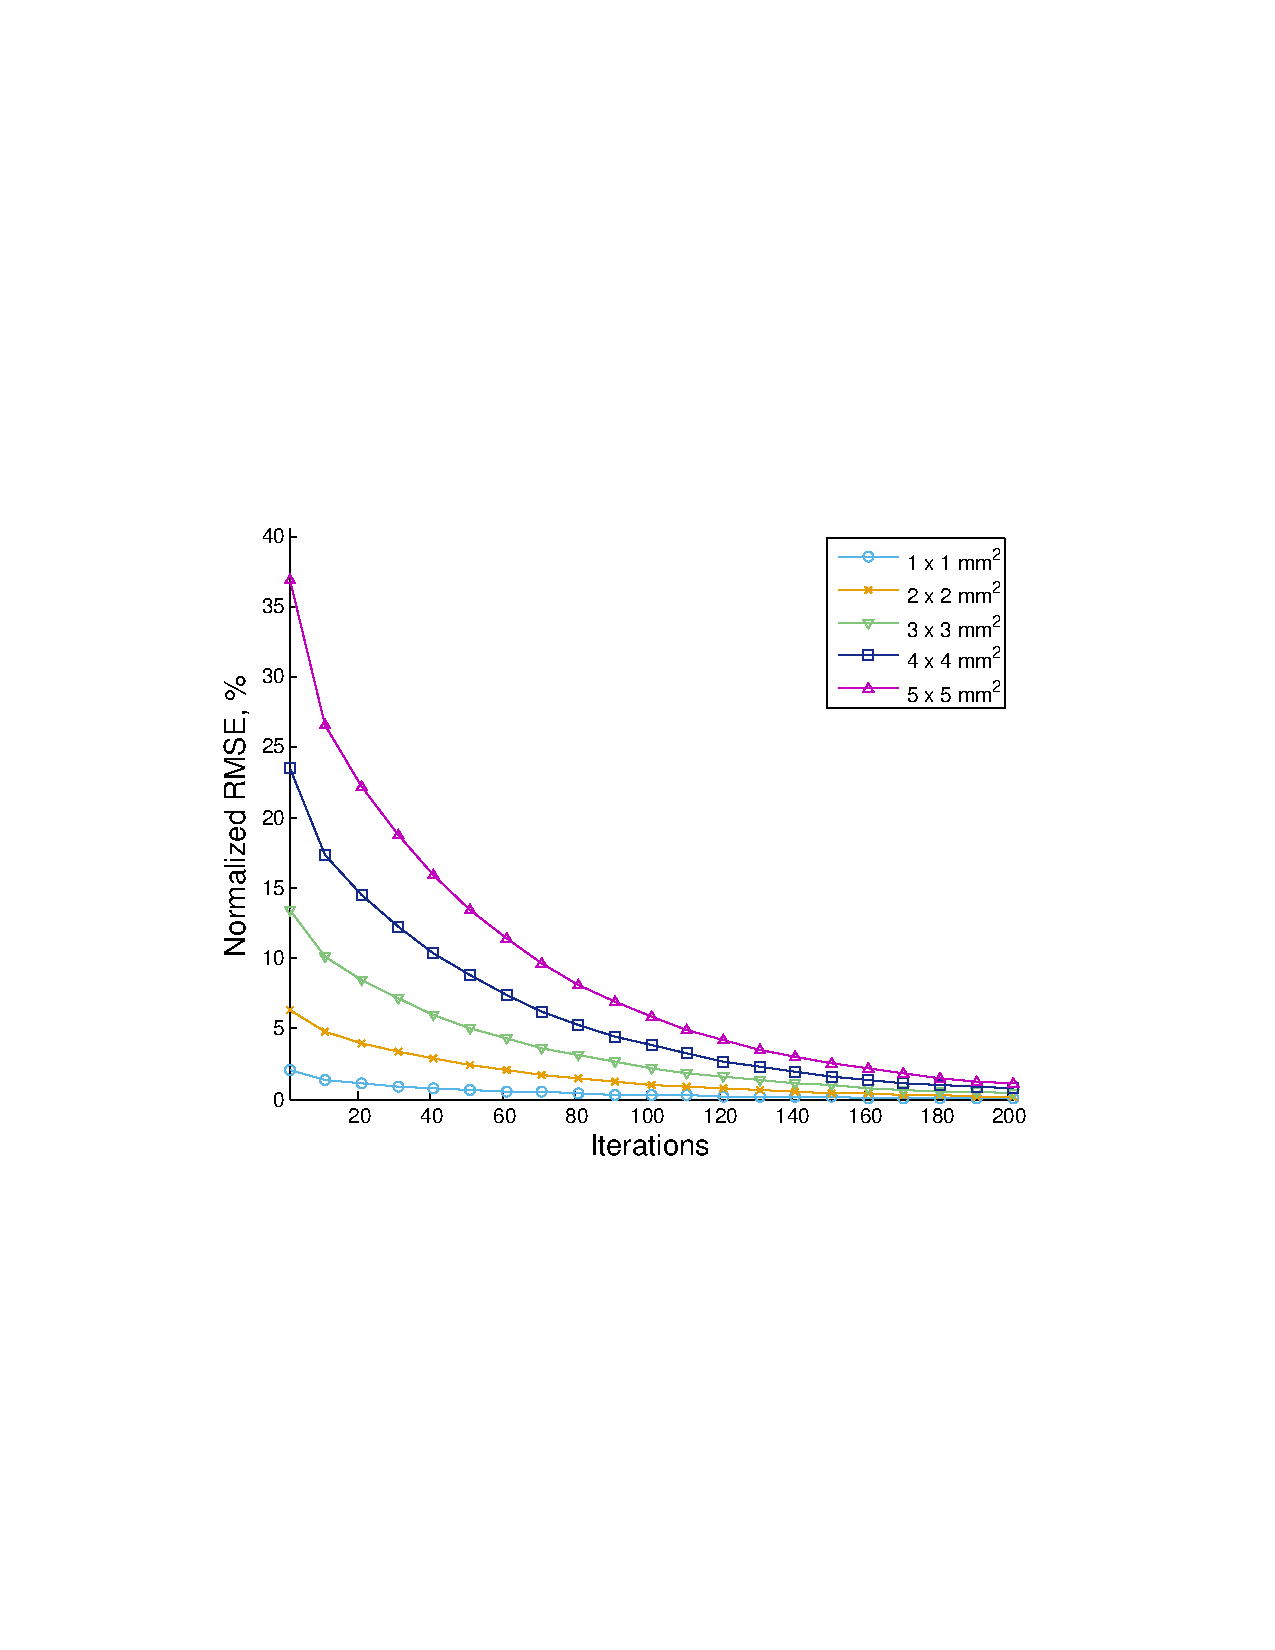
\includegraphics[width=0.32\linewidth]{assets/hotspot-error.pdf}
  }
  \subfloat[An example of the SSA.]{
    \label{fig:steady-state-approximation}
    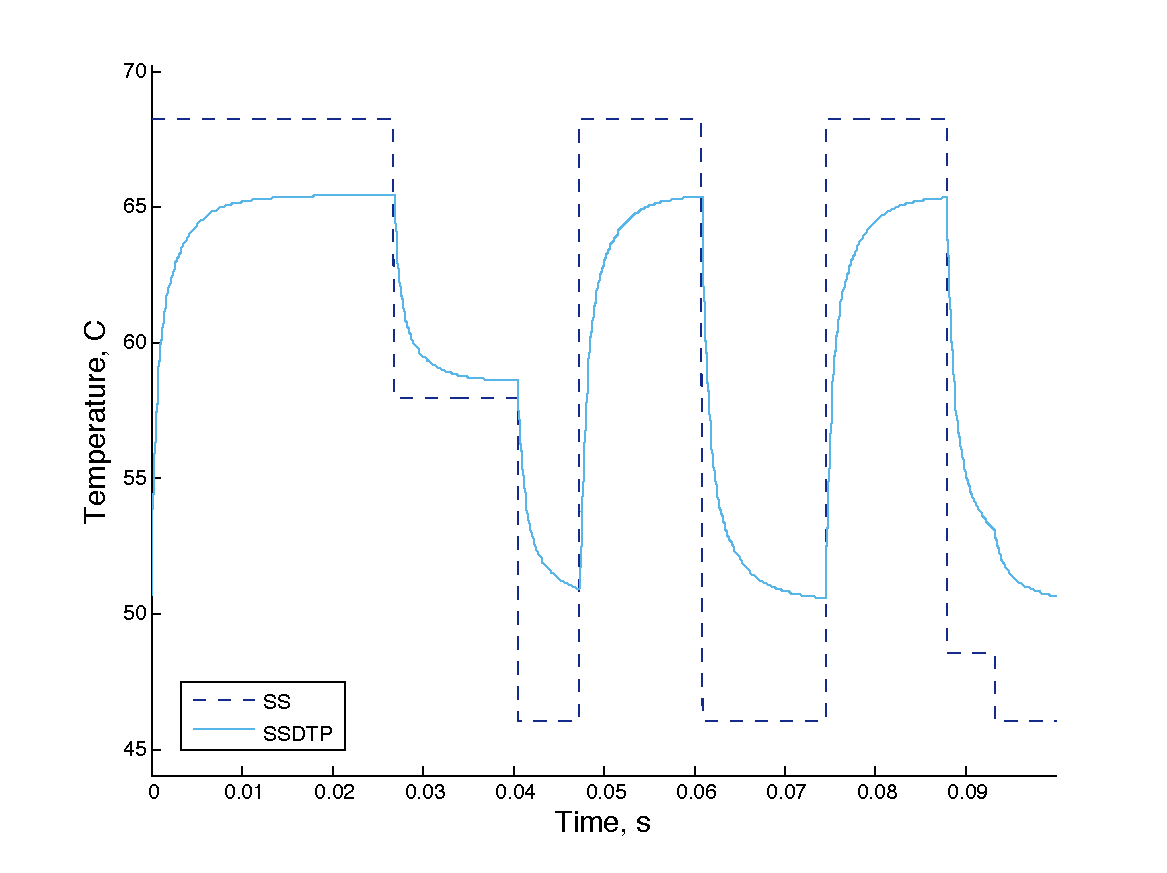
\includegraphics[width=0.32\linewidth]{assets/steady-state-approximation.pdf}
  }
  \subfloat[The NRMSE of the SSA.]{
    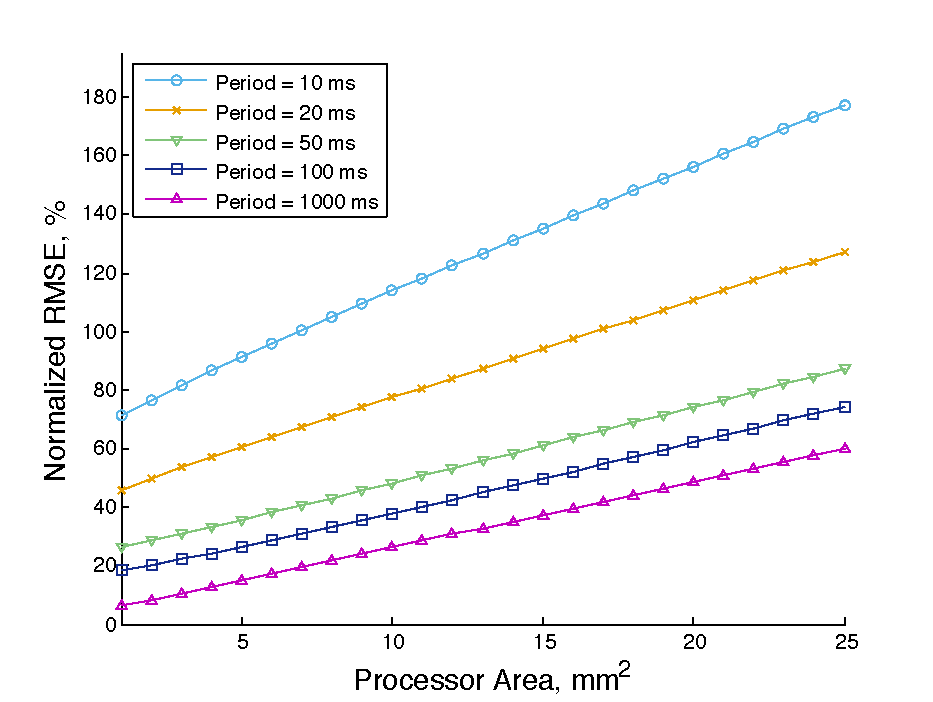
\includegraphics[width=0.32\linewidth]{assets/steady-state-error.pdf}
    \label{fig:steady-state-error}
  }
  \caption{State of the art solutions.}
\end{figure*}

\begin{itable}{parameters}{|l|r|}
  {Parameters of the Die and Thermal Package.}
  {The thermal parameters (i.e., thermal conductivity, specific heat, convection resistance and capacitance) used in our experiments are equal to the default ones found in HotSpot 5.0 \cite{huang2003}.}
  \hline
  Parameter & Value \\
  \hline
  \hline
  Ambient temperature                   &   27 ${}^\circ C$ \\
  Convection capacitance                & 140.4 J/K \\
	Convection resistance                 & 0.1 K/W \\
  Die thickness                         & 0.15 $mm$ \\
  Thermal interface material thickness  & 0.02 $mm$ \\
  Heat spreader side                    &   20 $mm$ \\
  Heat spreader thickness               &    1 $mm$ \\
  Heat sink side                        &   30 $mm$ \\
  Heat sink thickness                   &   15 $mm$ \\
  \hline
\end{itable}
The number of simulations required to reach the SSDTP depends on the thermal characteristics of the system. In order to illustrate this aspect, we have considered an application with the period of 0.5 seconds running on five hypothetical platforms with core areas between 1 and 25 $mm^2$. The configuration of the die itself and thermal package is given in \tabref{tab:parameters}. We have run the temperature simulation with HotSpot \cite{huang2003} for 50 successive periods of the application. The temperature profile in each period has been compared with the real SSDTP obtained with our analytical approach (\secref{sec:analytical-solution}) and the normalized Root Mean Square Error (RMSE) has been calculated. The result is shown in \figref{fig:hotspot-error}. It can be observed that the number of successive periods over which the temperature simulation has to be performed in order to achieve a satisfactory level of accuracy is significant for the majority of configurations. For a 9 $mm^2$ die, for example, after 15 iterations, the normalized RMSE is still close to 20\%. This leads to large computation times, making it difficult to apply the technique inside an intensive optimization loop.

\subsection{Steady-State Approximation (SSA)} \label{sec:steady-state-approximation}
An approximation method of the SSDTP has been proposed in \cite{huang2009}. Instead of solving the system of differential equations given by \equref{eq:fourier-model}, it is assumed that during each time interval $\Delta t_i$ in which the power is constant the whole system stays in its steady state. In this case the derivative \mbox{$d\v{T}/dt = 0$} and the temperature can be calculated as $\v{T}_i = \m{G}^{-1} \v{P}_i$.

The result is a stepwise temperature curve where each step corresponds to the steady-state temperature $\v{T}_i$ that would be reached if the constant power $\v{P}_i$ was applied for a sufficiently long time. An example of such an approximation (SSA) along with the corresponding SSDTP for an application with 10 tasks and period of 0.1 seconds is given in \figref{fig:steady-state-approximation}. The die area is 25 $mm^2$, the configuration of the chip is the same as in \tabref{tab:parameters}. The reduced accuracy of the approximation is due to the mismatch between the actual temperature within each interval $\Delta t_i$ and the hypothetical steady-state temperature. The inaccuracy depends on the thermal characteristics of the respective platform and on the application itself. To illustrate this, we have generated five applications with periods between 0.01 and 1 seconds and computed approximated SSDTPs for die areas between 1 and 25 $mm^2$. The normalized RMSE relative to the correct SSDTP is shown in \figref{fig:steady-state-error}. It can be seen that, e.g., for a die area of 10 $mm^2$ and a period of 100 $ms$ the normalized RMSE with the SSA is close to 40\%.
